\documentclass{article}

\usepackage{amsmath, amsthm}
\usepackage{setspace}
\usepackage{microtype, parskip}
\usepackage[comma,sort&compress]{natbib}
\usepackage{lineno}
\usepackage{docmute}
\usepackage{caption, subcaption, multirow, morefloats, rotating}
\usepackage{wrapfig}

\frenchspacing

\doublespacing

\raggedright

\begin{document}
\linenumbers
\modulolinenumbers[2]

%\maketitle

\begin{titlepage}
  \begin{large}
    \textbf{Title:} How do biological traits affect brachiopod taxonomic survival? A hierarchical Bayesian approach.
  \end{large}

  \textbf{Running title:} How do biological traits affect taxonomic survival?

  \textbf{Author:} Peter D Smits, psmits@uchicago.edu, Committee on Evolutionary Biology, University of Chicago

  \textbf{Keywords:} extinction, macroevolution, macroecology, Paleozoic, selection

  \textbf{Word count:} ?
  
  \textbf{Table count:} 0.
 
  \textbf{Figure count:} 5 main text, 3 supplement.

  \textbf{Data archival location:} If accepted, all data and code necessary to duplicate this analysis will be made available on DRYAD.

\end{titlepage}

\documentclass[12pt,letterpaper]{article}

\usepackage{amsmath, amsthm}
\usepackage{microtype, parskip}
\usepackage[comma,numbers,sort&compress]{natbib}
\usepackage{lineno}
\usepackage{docmute}
\usepackage{caption, subcaption, multirow, morefloats, rotating}
\usepackage{wrapfig}

\frenchspacing

\captionsetup[subfigure]{position = top, labelfont = bf, textfont = normalfont, singlelinecheck = off, justification = raggedright}

\begin{document}

\begin{abstract}
  While the effect of geographic range on extinction risk is well documented, the effects of other traits are less well known. Using a hierarchical Bayesian modeling approach, I also model the possible interaction between the effects of the biological traits and a taxon's time of origination. I analyze patterns of Paleozoic brachiopod genus durations and their relationship to geographic range, affinity for epicontinental seas versus open ocean environments, and body size. Additionally, I allow for environmental affinity to have a nonlinear effect on duration. My analysis framework eschews the traditional distinction between background and mass extinction, instead the entire time period is analyzed where these ``states'' are part of a continuum. I find evidence that as extinction risk increases, the expected strength of the selection gradient on biological traits (except body size) increases. This manifests as greater expected differences in extinction risk for each unit change in geographic range and environmental preference during periods of high extinction risk, as opposed to a much flatter expected selection gradient during periods of low extinction risk. I find weak evidence for a universally nonlinear relationship between environmental preference and extinction risk such that ``generalists'' have a lower expected extinction risk than either ``specialists''. While for the many parts of the Paleozoic this hypothesis is supported, there are many times where this hypothesized relationship is absent or even reversed. Importantly, I find that as extinction risk increases, the steepness of this relationship is expected to increases as well.
\end{abstract}

\end{document}


\documentclass[12pt,letterpaper]{article}

\usepackage{amsmath, amsthm}
\usepackage{microtype, parskip}
\usepackage[comma,numbers,sort&compress]{natbib}
\usepackage{lineno}
\usepackage{docmute}
\usepackage{caption, subcaption, multirow, morefloats, rotating}
\usepackage{wrapfig}

\frenchspacing

\captionsetup[subfigure]{position = top, labelfont = bf, textfont = normalfont, singlelinecheck = off, justification = raggedright}

\begin{document}
\section{Introduction}

How do biological traits affect extinction risk? \citet{Jablonski1986} observed that during periods of high extinction risk, the effects of biological traits on survival decreased in size. However, this pattern was weakest/absent in the effect of geographic range on survival \citep{Jablonski1986}. Biological traits are defined here as descriptors of a taxon's adaptive zone, which is the set of biotic--biotic and biotic--abiotic interactions that a taxon can experience \citep{Simpson1944}. In effect, these are descriptors of a taxon's broad-sense ecology.

\citet{Jablonski1986} phrased his conclusions in terms of background versus mass extinction, but this scenario is readily transferable to a continuous variation framework as there is no obvious distinction in terms of extinction rate between these two states \citep{Wang2003}. Additionally, the \citet{Jablonski1986} scenario has strong model structure requirements in order to test its proposed macroevolutionary mechanism; not only do the taxon trait effects need to be modeled, but the correlation between the trait effects need to be modeled as well. 

There are two end-member macroevolutionary mechanisms which may underlie the pattern observed by \citet{Jablonski1986}: the effect of geographic range on predictive survival remains constant and those of other biological traits decrease, and the effect of geographic range in predicting survival increases and those of other biological traits stay constant. Reality, of course, may fall somewhere along the continuum between these two opposites.

I model brachiopod taxon durations because trait based differences in extinction risk should manifest as differences in taxon durations. Namely, a taxon with a beneficial trait should survive longer, on average, than a taxon without that beneficial trait. Conceptually, taxon survival can be considered an aspect of ``taxon fitness'' along with expected lineage specific branching/origination rate \citep{Cooper1984,Palmer2012}. Brachiopods are an ideal group for this study as they are are well known for having an exceptionally complete fossil records \citep{Foote2000a}. Specifically, I focus on the brachiopod record from most of the Paleozoic, specifically from the start of the Ordovician (approximately 485 Mya) through the end Permian (approximately 252 Mya) as this represents the time of greatest global brachiopod diversity \citep{Alroy2010}.

he analysis of taxon durations, or time from origination to extinction, falls under the purview of survival analysis, a field of applied statistics commonly used in health care \citep{Klein2003} but has a long history in paleontology \citep{Simpson1944,Simpson1953,VanValen1973,VanValen1979}.

Geographic range is widely considered the most important taxon trait for estimating differences in extinction risk at nearly all times with large geographic range associated with low extinction risk \citep{Jablonski1986,Jablonski1987,Jablonski2003,Payne2007}. I expect this to hold true nearly always.

\citet{Miller2009a} demonstrated that during several mass extinctions taxa associated with open-ocean environments tend to have a greater extinction risk than those taxa associated with epicontinental seas. During periods of background extinction, however, they found no consistent difference between taxa favoring either environment. These two environment types represent the primary environmental dichotomy observed in ancient marine systems \citep{Miller2009a,Peters2008,Sheehan2001b}. 

Epicontinental seas are a shallow-marine environment where the ocean has spread over the surface of a continental shelf with a depth typically less than 100m. In contrast, open-ocean coastline environments have much greater variance in depth, do not cover the continental shelf, and can persist during periods of low sea level. Because of this, it is strongly expected that taxa which favor epicontinental seas would be at great risk during periods of low sea levels, such as during glacial periods, where these seas are drained. During the Paleozoic (approximately 541--252 My), epicontinental seas were widely spread globally but declined over the Mesozoic (approximately 252--66 My) and eventually diminished disappearing during the Cenozoic (approximately 66--0 My) as open-ocean coastlines became the dominant shallow-marine setting \citep{Peters2008,Miller2009a,Johnson1974}. 

Given the above information, I predict that as extinction risk increases, taxa associated with open-ocean environments should generally increase in extinction risk versus those that favor epicontinental seas. Additionally, there is a possible nonlinear relationship between environmental preference and taxon duration. A long standing hypothesis is that generalists or unspecialized taxa will have greater survival than specialists \citep{Simpson1944,Liow2004a,Liow2007b,Nurnberg2013a,Nurnberg2015,Baumiller1993}. In this analysis I allowed for environmental preference to possibly have a parabolic effect on taxon duration 

Body size, measured as shell length \citep{Payne2014}, was also considered as a potentially informative covariate. Body size is a proxy for metabolic activity and other correlated life history traits \citep{Payne2014}. There is no strong hypothesis of how body size effects extinction risk in brachiopods, meaning a positive, negative, or zero effect are all plausible. 

I adopt a hierarchical Bayesian survival modeling approach, which represents a conceptual and statistical unification of the paleontological dynamic and cohort survival analytic approaches \citep{VanValen1973,VanValen1979,Raup1978,Raup1975,Foote1988,Baumiller1993,Simpson2006}. By using a Bayesian framework I am able to quantify the uncertainty inherent in the estimates of the effects of biological traits on survival, especially in cases where the covariates of interest (i.e. biological traits) are themselves known with error. 

\end{document}


\documentclass[12pt,letterpaper]{article}

\usepackage{amsmath, amsthm}
\usepackage{microtype, parskip}
\usepackage[comma,numbers,sort&compress]{natbib}
\usepackage{lineno}
\usepackage{docmute}
\usepackage{caption, subcaption, multirow, morefloats, rotating}
\usepackage{wrapfig}

\frenchspacing

\begin{document}
\section{Materials and Methods}
\subsection{Taxon occurrence information}
The dataset analyzed here was sourced from the Paleobiology Database (http://www.paleodb.org) which was then filtered based on taxonomic, temporal, stratigraphic, and other occurrence information that was necessary for this analysis. These filtering criteria are very similar to those from \citet{Foote2013}.

Fossil occurrences were analyzed at the genus level which is common for paleobiological, macroevolutionary, or macroecological studies of marine invertebrates \citep{Alroy2010,Foote2013,Harnik2013,Kiessling2007a,Miller2009a,Nurnberg2013a,Nurnberg2015,Payne2007,Simpson2009,Vilhena2013}. Although species diversity dynamics tend to be of much greater interest than those of higher taxa, the nature of the fossil record makes accurate and precise taxonomic assignments at the species level for all occurrences extremely difficult if not impossible. Additionally, there is evidence of real differences in biological patterns at the genus level versus the species level \citep{Jablonski1987}. As such, the choice to analyze genera as opposed to species was in order to assure a minimum level of confidence and accuracy in the data analyzed here.

Geographic regions were defined by dividing the globe into four latitudinal bands at the equator and both the tropics of Cancer and Capricorn (\(\pm 23.5^\circ\)). These boundary lines were chosen because they are defined independent of taxonomic occurrence and are constant throughout they are defined independent of taxonomic occurrence and are spatially constant throughout time. Tectonic plates, for example, while geologically constant are not spatially constant. Given that latitudinal diversity gradients are one of the focuses of this study, using spatially variable regions is inappropriate given that a given plate my transition from tropical to temperate or vice-versa.


\subsection{Model specification}
Taxon presence was modeled has a hierarchical hidden Markov model (HMM) where the three ``process parameters'' of gain/newly entering a province (\(\gamma\)), persistance/survival (\(\phi\)), and observation (\(p\)). For each province, each of these process parameters were modeled hierarchically so that estimates were allowed to vary over time but in cases of little information those estimates were drawn to the overall mean for that province. The estimates for each province were also estimated hierarchically in relation to each other; this way all estimates were relative to each other. The hierarchical structure of this model helps control for both overfitting and multiple comparisons during posterior analysis \citep{Gelman2007,Gelman2013d}. 

Note that the following model is strongly inspired by the dynamic occupancy model presented in \citep{Royle2008}.

\(y_{i, j, t}\) is the observed occurrence of taxon \(i\) in province \(j\) at time \(t\), where \(i = 1, 2, \dots, N\), \(j = 1, 2, \dots, J\), and \(t = 1, 2, \dots, T\). \(y = 1\) is occupied while \(y = 0\) is unoccupied. \(z_{i, j, t}\) is the ``true'' occurrence of taxon \(i\) in province \(j\) at time \(t\), given the estimate of sampling. Just as with \(y\), \(z = 1\) is occupied while \(z = 0\) is unoccupied. 

\(\phi_{j, t}\) is the probability of surviving, in province \(j\), from time \(t\) to time \(t + 1\) (\(Pr(z_{t + 1} = 1 | z_{t} = 1)\)). \(\gamma_{j, t}\) is the probability of newly entering province \(j\) at time \(t + 1\) (\(Pr(z_{t + 1} = 1 | z_{t} = 0)\)). \(p_{j, t}\) is the probability of observing a true occurrence (\(Pr(y = 1 | z = 1)\)) in province \(j\) at time \(t\). 

\(\psi\) is probability of sit occupancy/probability of occurrence (\(Pr(z_{i, t = 1} = 1)\). The first time point is defined in terms of \(\psi\) because there is (assumed) no previous time points.

The parameters \(\phi\), \(\gamma\), and \(p\) are then all defined hierarchically within time bins as samples from the shared mean between provinces. \(\Phi_{t}\), \(\Gamma_{t}\), and \(P_{t}\) are the mean probabilities for a given point in time \(t\). \(M_{\phi}\), \(M_{\gamma}\), and \(M_{p}\) are the overall mean estimates of survival, origination, and preservation probabilities. 

And finally, I use independent uniform priors for \(\psi_{j}\) by province \(j\): \(\psi_{j} \sim \mathrm{U}(0, 1)\).

In total, the model can be summarized by the following statements:

\begin{equation}
  \begin{aligned}
    y_{i, t, j} &\sim \mathrm{Bern}(p_{t, j} z_{i, t, j}) \\
    z_{i, t = 1, j} &\sim \mathrm{Bern}(\psi_{j}) \\
    z_{i, t, j} &\sim \mathrm{Bern}(\phi_{j, t - 1} z_{i, t - 1, j} + \gamma_{j, t - 1} (1 - z_{i, t - 1, j})) \\
    \mathrm{logit}(\phi_{j, t}) &\sim \mathrm{N}(\Phi_{t}, \sigma_{\phi, t}) \\
    \mathrm{logit}(\gamma_{j, t}) &\sim \mathrm{N}(\Gamma_{t}, \sigma_{\gamma, t}) \\
    \mathrm{logit}(p_{j, t}) &\sim \mathrm{N}(P_{t}, \sigma_{p, j}) \\
    \Phi_{i} &\sim \mathrm{N}(M_{\phi}, \sigma_{\Phi}) \\
    \Gamma_{i} &\sim \mathrm{N}(M_{\gamma}, \sigma_{\Gamma}) \\
    P_{i} &\sim \mathrm{N}(M_{p}, \sigma_{P}) \\
    \sigma_{\phi, i} &\sim \mathrm{C}^{+}(1) \\
    M_{\phi} &\sim \mathrm{N}(0, 1) \\
    \sigma_{\Phi} &\sim \mathrm{C}^{+}(1) \\
    \sigma_{\gamma, j} &\sim \mathrm{C}^{+}(1) \\
    M_{\gamma} &\sim \mathrm{N}(0, 1) \\
    \sigma_{\Gamma} &\sim \mathrm{C}^{+}(1) \\
    \sigma_{p, j} &\sim \mathrm{C}^{+}(1) \\
    M_{p} &\sim \mathrm{N}(0, 1) \\
    \sigma_{P} &\sim \mathrm{C}^{+}(1) \\
  \end{aligned}
\end{equation}


\subsection{Posterior inference}
The joint posterior distribution of the HMM model was approximated using a Gibbs sampling MCMC routine as implemented in the JAGS probabilistic programming language CITATION. Four chains were each run for 100000 steps, thined to every 100th sample, and split evenly between warm-up and sampling phases. Chain sampling convergence was assessed using the \(\hat{R}\) statistic with values close to 1 (less than 1.1) indicating approximate convergence \citep{Gelman2013d}.

% assessing model fit
%   posterior predictive check
%     simulate time series starting from t = 1
%     compare observed to simulated
% 80 / 20 split
%   take a random 20% sample of taxa and set aside as ``test set''
%   fit the model to the remaining 80% ``training set''
%   after the model is fit, try to predict the observed pattern of test set


% posterior inference
% turnover
% is this actually necessary as an estimate?
%   would be extremely difficult to explain to a paleontological audience when they are thinking of a ratio of per captia rates and this is a probability.
%   estimate number of 0 --> 1 changes (gains) and number of 1 --> 0 changes (losses) from time t to t - 1.
%     already have the diversity estimate of each point in time.

Given the estimate of the joint posterior distribution, some downstream metapopulation summary statistics can be calculated. Given the estimates of \(z\) it is trivial to calculate the number of taxa that newly enter or exit any region \(j\) at any time \(t\). Additionally, the net change in taxonomic diversity (entrances minus exits) can be calculated for any region \(j\) at any time \(t\).

Turnover \(\tau\) defined as the probability that the occurrence of a taxon at time \(t\) is new (\(Pr(z_{t - 1} = 0 | z_{t} = 1)\)) \citep{Royle2008}. First, the occupancy probability \(\psi\) at times \(t = 2, \dots, T\) can calculated recursively as
\begin{equation}
  \psi_{t} = \psi_{t - 1}\phi_{t - 1} + (1 - \psi_{t - 1})\gamma_{t - 1}.
\end{equation}
Turnover can then be calculated as
\begin{equation}
  \tau_{t} = \frac{\gamma_{t - 1} (1 - \gamma_{t - 1}}{\gamma_{t - 1} (1 - \psi_{t - 1}) + \phi_{t - 1} \psi_{t - 1}}.
\end{equation}
An additional summary is the growth rate \(\lambda\) \citep{MacKenzie2003,Royle2008} which is calculated as
\begin{equation}
  \lambda_{t} = \frac{\psi_{t + 1}}{\psi_{t}}.
\end{equation}

% what does this mean?
%The final summary static of interest is the equilibrium occupancy probability \citep{MacKenzie2006,Royle2008}
%\begin{equation}
%  \psi_{t}^{\text{eq}} = \frac{\gamma_{t}}{\gamma_{t} + (1 - \phi_{t})}
%\end{equation}

\end{document}


\documentclass[12pt,letterpaper]{article}

\usepackage{amsmath, amsthm}
\usepackage{microtype, parskip}
\usepackage[comma,numbers,sort&compress]{natbib}
\usepackage{lineno}
\usepackage{docmute}
\usepackage{caption, subcaption, multirow, morefloats, rotating}
\usepackage{wrapfig}

\frenchspacing

\captionsetup[subfigure]{position = top, labelfont = bf, textfont = normalfont, singlelinecheck = off, justification = raggedright}

\begin{document}
\section{Results}

As stated above, posterior approximations for both the exponential and Weibull models achieved approximate stationarity after 10,000 steps, as all parameter estimates have an \(\hat{R} < 1.1\).%\uppercase{ref tables}.

Comparisons of the survival functions estimated from 1000 posterior predictive data sets to the estimated survival function of the observed genera demonstrates that both the exponential and Weibull models approximately capture the observed pattern of extinction (Fig. \ref{fig:surv}). The major difference in fit between the two models is that the Weibull model has a slightly better fit for longer lived taxa than the exponential model.

%Inspection of the deviance residuals yields a similar pattern of biased estimates for longer lived taxa \uppercase{ref figure}. 

Additionally, the Weibull model is expected to have slightly better out-of-sample predictive accuracy when compared to the exponential model (WAIC 4576 versus 4604, respectively). \ref{fig:surv}). Because the difference in WAIC between these two models is large, while results from both the exponential and Weibull models will be presented, only those from the Weibull model will be discussed.

% Results/hypothesis tests
%   \mu of hierarchical effects
%   \tau of hierarchical effects (partial pooling)
Estimates of the overall mean covariate effects \(\mu\) can be considered time-invariant generalizations for brachiopod survival during the Paleozoic (Fig. \ref{tab:param}). Consistent with prior expectations, geographic range size has a negative effect on extinction risk, where genera with large ranges having greater durations than genera with small ranges. 

I find that while the mean estimate of the effect of body size on extinction risk is negative, implying that increasing body size decreases extinction risk, this estimate is within 2 standard deviations of 0 (mean \(\mu_{m} = -0.09\), standard deviation 0.09; Fig. \ref{tab:param}). Because of this, I infer that body size has no distinguishable effect on brachiopod taxonomic survival.

Interpretation of the effect of environmental preference \(v\) on duration is slightly more involved. Because a quadratic term is the equivalent of an interaction term, both \(\mu_{v}\) and \(\mu_{v^{2}}\) have to be interpreted together because it is illogical to change values of \(v\) without also changing values \(v^{2}\). To determine the nature of the effect of \(v\) on duration I calculated the multiplicative effect of environmental preference on extinction risk.

Given mean estimated extinction risk \(\tilde{\sigma}\), we can define the extinction risk multiplier of an observation with environmental preference \(v_{i}\) as 
\begin{equation}
  \frac{\tilde{\sigma_{i}}}{\tilde{\sigma}} = f(v_{i}) = \exp\left(\frac{-(\mu_{v} v_{i} + \mu_{v^{2}} v^{2})}{\alpha}\right).
  \label{eq:env}
\end{equation}
This function \(f(v_{i})\) has a y-intercept of \(\exp(0)\) or 1 because it does not have a non-zero intercept term. Equation \ref{eq:env} can be either concave up or down. A concave down \(f(v_{i})\) may indicate that genera of intermediate environmental preference have greater durations than either extreme, and \textit{vice versa} for concave up function.

The expected effect of environmental preference as a multiplier of expected extinction risk can then be visualized (Fig. \ref{fig:env_mean}). This figure depicts 1000 posterior predictive estimates of Eq. \ref{eq:env} across all possible values of \(v\). The number indicates the posterior probability that the function is concave down, with generalists having lower extinction risk/greater duration than either type of specialist. Note that the inflection point/optimum of Fig. \ref{fig:env_mean} is approximately \(x = 0\), something that is expected given the estimate of \(\mu_{v}\) (Fig. \ref{tab:param}).

The matrix \(\Sigma\) describing the covariance between the different coefficients describes how these coefficients might vary together across the origination cohorts. Similar to how this was modeled (Eq. \ref{eq:exp_total}, \ref{eq:wei_total}), for interpretation purposes \(\Sigma\) can be decomposed into a vector of standard deviations \(\vec{\tau}\) and a correlation matrix \(\Omega\).

The estimates of the standard deviation of between-cohort coefficient estimates \(\tau\) inidicate that some effects can vary greatly between-cohorts (Fig. \ref{tab:param}). Coefficients with greater values of \(\tau\) have greater between-cohort variation. The covariate effects with the greatest between origination cohort variation are \(\beta_{r}\), \(\beta_{v}\), and \(\beta_{v^{2}}\). Estimates of \(\beta_{m}\) have negligible between cohort variation, as there is less between cohort variation than the between cohort variation in baseline extinction risk \(\beta_{0}\). However the amount of between cohort variation in estimates of \(\beta_{v^{2}}\) means that it is possible for the function describing the effect of environmental affinity to be upward facing for some cohorts (Eq. \ref{eq:env}), which corresponds to environmental generalists being shorter lived than specialists in that cohort.


% omega heatmap
%   correlations with baseline extinction risk of of major interest
%   high/positive values of intercept --> high extinction risk
%   low/negative values of intercept --> low extinction risk
The correlation terms of \(\Omega\) (Fig. \ref{fig:omega}) describe the relationship between the coefficients and how their estimates may vary together across cohorts. The correlations between the intercept term \(\beta_{0}\) and the effects of the taxon traits are of particular interest for evaluating the \citet{Jablonski1986} scenario (Fig. \ref{fig:omega} first column/last row). Keep in mind that when \(\beta_{0}\) is low, extinction risk is low; and conversely, when \(\beta_{0}\) is high, then extinction risk is high.

Marginal posterior probabilities of the correlations between the level of baseline extinction risk \(\beta_{0}\) and the effects of the taxon traits indicate that the correlation between expected extinction risk and both geographic range \(\beta_{r}\) and \(\beta_{v^{2}}\) are of particular note (Fig. \ref{fig:corr}). 

There is approximately a 98\% probability that \(\beta_{0}\) and \(\beta_{r}\) are negatively correlated (Fig. \ref{fig:corr}), meaning that as extinction risk increases, the effect/importance of geographic range on genus duration increases. This means that increases in baseline extinction rate are correlated with an increased importance of geographic range size. There is a 93\% probability that \(\beta_{0}\) and \(\beta_{v^{2}}\) are negatively correlated (Fig. \ref{fig:corr}), meaning that as extinction risk increases, the peakedness of \(f(v_{i})\) increases and the relationship tends towards concave down. Additionally, there is a 97\% probability that values of \(\beta_{r}\) and \(\beta_{v^{2}}\) are positively correlated (Mean correlation 0.51, standard deviation 0.23).

% effects varying between cohorts
While the overall group level estimates are of particular importance when defining time-invariant differences in extinction risk, it is also important and useful to analyze the individual level parameter estimates in order to better understand how parameters actually vary across cohorts.

In comparison to the overall mean extinction risk \(\mu_{0}\), cohort level estimates \(\beta_{0}\) show some amount of variation through time as expected by estimates of \(\tau_{0}\) (Fig. \ref{fig:cohort_intercept}). A similar, if slightly greater, amount of variation is also observable in cohort estimates of the effect of geographic range \(\beta_{r}\) (Fig. \ref{fig:cohort_range}). Again, smaller values of \(\beta_{0}\) correspond to lower expected extinction risk. Similarly, smaller values of \(\beta_{r}\) correspond to greater decrease in extinction risk with increasing geographic range 

% environmental effect for cohort
%   effect of environmental preference as duration multiplier
How the effect of environmental affinity varies between cohorts can be observed by using the cohort specific coefficients estimates. Following the same procedure used earlier (Fig. \ref{tab:param}), but substituting cohort specific estimates of \(\beta_{v}\) and \(\beta_{v^{2}}\) for \(\mu_{v}\) and \(\mu_{v^{2}}\), the cohort specific effect of environmental preference as a multiplier of mean extinction risk can be calculated. This was done only for the Weibull model, though the observed pattern should be similar for the exponential model. 

As expected based on the estimates of \(\tau_{v}\) and \(\tau_{v^{2}}\), there is greater variation in the peakedness of \(f(v_{i})\) than there is variation between convave up and down functions (Fig. \ref{fig:env_cohort}). 12 of the 33 cohorts have less than 50\% posterior probability that generalists are potentially expected to be shorter lived than specialists, though two of those cases have approximately a 50\% probability of being either concave up or down. This is congruent with the 0.72 posterior probability that \(\mu_{v^{2}}\) is positive/\(f(v_{i})\) is concave down.


Additionally, for some cohorts there is a quite striking pattern where the effect of environmental preference \(v\) has a nearly-linear relationship (Fig. \ref{fig:env_cohort}). These are primarily scenarios where one of the end member preferences is expected to have a greater duration than either intermediate or the opposite end member preference. Whatever curvature is present in these nearly-linear cases is due to the defintion of \(f(v)\) as it is not defined for non-negative values of \(\sigma\) (Eq. \ref{eq:env}). For all stages between the Emsian through the Vis\'{e}an, inclusive, intermediate preferences are of intermediate extinction risk when compared with epicontinental specialists (lowest risk) or open-ocean specialists (highest risk). This time period represents most of the Devonian through the early Carboniferous.

\end{document}


\documentclass[12pt,letterpaper]{article}

\usepackage{amsmath, amsthm}
\usepackage{microtype, parskip}
\usepackage[comma,numbers,sort&compress]{natbib}
\usepackage{lineno}
\usepackage{docmute}
\usepackage{caption, subcaption, multirow, morefloats, rotating}
\usepackage{wrapfig}

\frenchspacing

\captionsetup[subfigure]{position = top, labelfont = bf, textfont = normalfont, singlelinecheck = off, justification = raggedright}

\begin{document}
\section{Discussion}

\end{document}


\section*{Acknowledgements}
I would like to thank K. Angielzcyk, M. Foote, P. D. Polly, and R. Ree for helpful discussion and advice. Additionally, thank you A. Miller for the epicontinental versus open-ocean assignments. This entire study would would not have been possible without the Herculean effort of the many contributors to the Paleobiology Database. In particular, I would like to thank J. Alroy, M. Aberhan, D. Bottjer, M. Clapham, F. F\"{u}rsich, N. Heim, A. Hendy, S. Holland, L. Ivany, W. Kiessling, B. Kr\"{o}ger, A. McGowan, T. Olszewski, P. Novack-Gottshall, M. Patzkowsky, M. Uhen, L. Villier, and P. Wager. This work was supported by a NASA Exobiology grant (NNX10AQ446) to A. Miller and M. Foote. This is Paleobiology Database publication XXX.

\clearpage

\bibliographystyle{evolution}
\bibliography{newbib,packages}

\clearpage

\begin{figure}[ht]
  \centering
  \includegraphics[height = 0.5\textheight,width=\textwidth,keepaspectratio=true]{figure/survival_curves}
  \caption{Comparison of empirical estimates of \(S(t)\) versus estimates from 1000 posterior predictive data sets. \(S(t)\) corresponds to \(P(T > t)\) as it is the probability that a given genus observed at age \(t\) will continue to live. This is equivalent to the probability that \(t\) is less than the genus' ultimate duration \(T\). Note that the Weibull (left) model has noticeably better fit to the data than the exponential (right).}
  \label{fig:surv}
\end{figure}

\begin{figure}[ht]
  \centering
  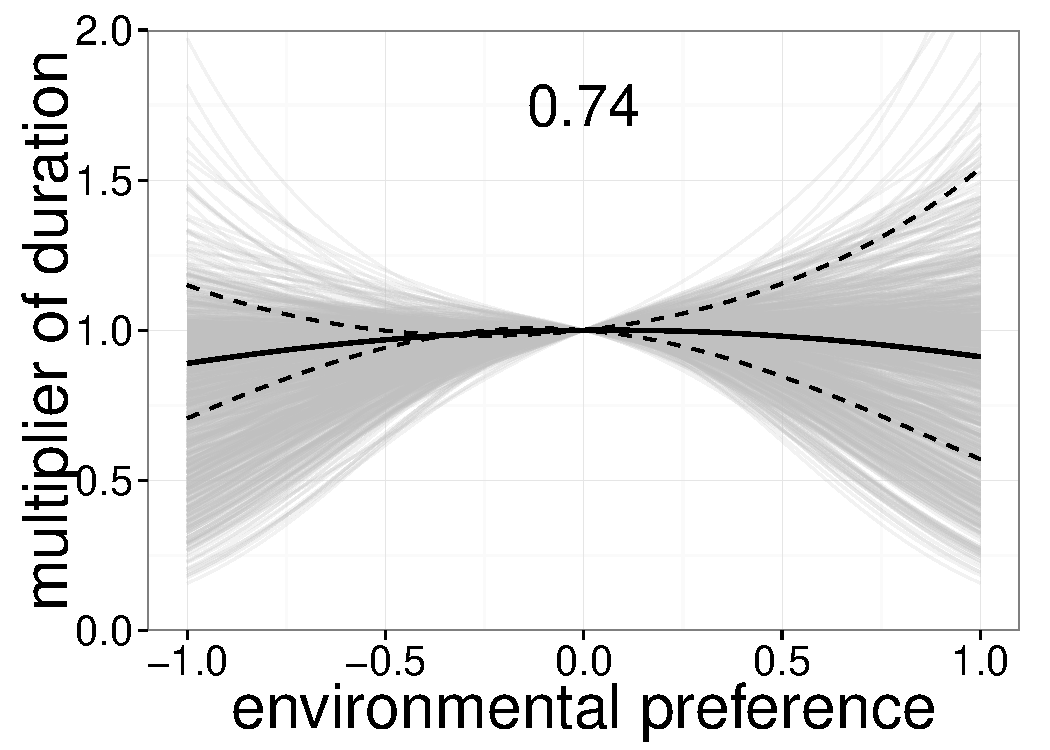
\includegraphics[height = 0.5\textheight,width=\textwidth,keepaspectratio=true]{figure/environ_quad}
  \caption{The overall expected relationship \(f(v_{i})\) between environmental affinity \(v_{i}\) and a multiplier of extinction risk (Eq. \ref{eq:env}). Each grey line corresponds to a single draw from the posterior predictive distribution, while the black corresponds to the median of the posterior predictive distribution. The overall shape of \(f(v_{i})\) is concave down with an optimum of close 0, which corresponds to affinity approximately equal to the expectation based on background environmental occurrence rates.}
  \label{fig:env_mean}
\end{figure}


\begin{figure}[ht]
  \centering
  \begin{subfigure}[b]{0.5\textwidth}
    \caption{}
    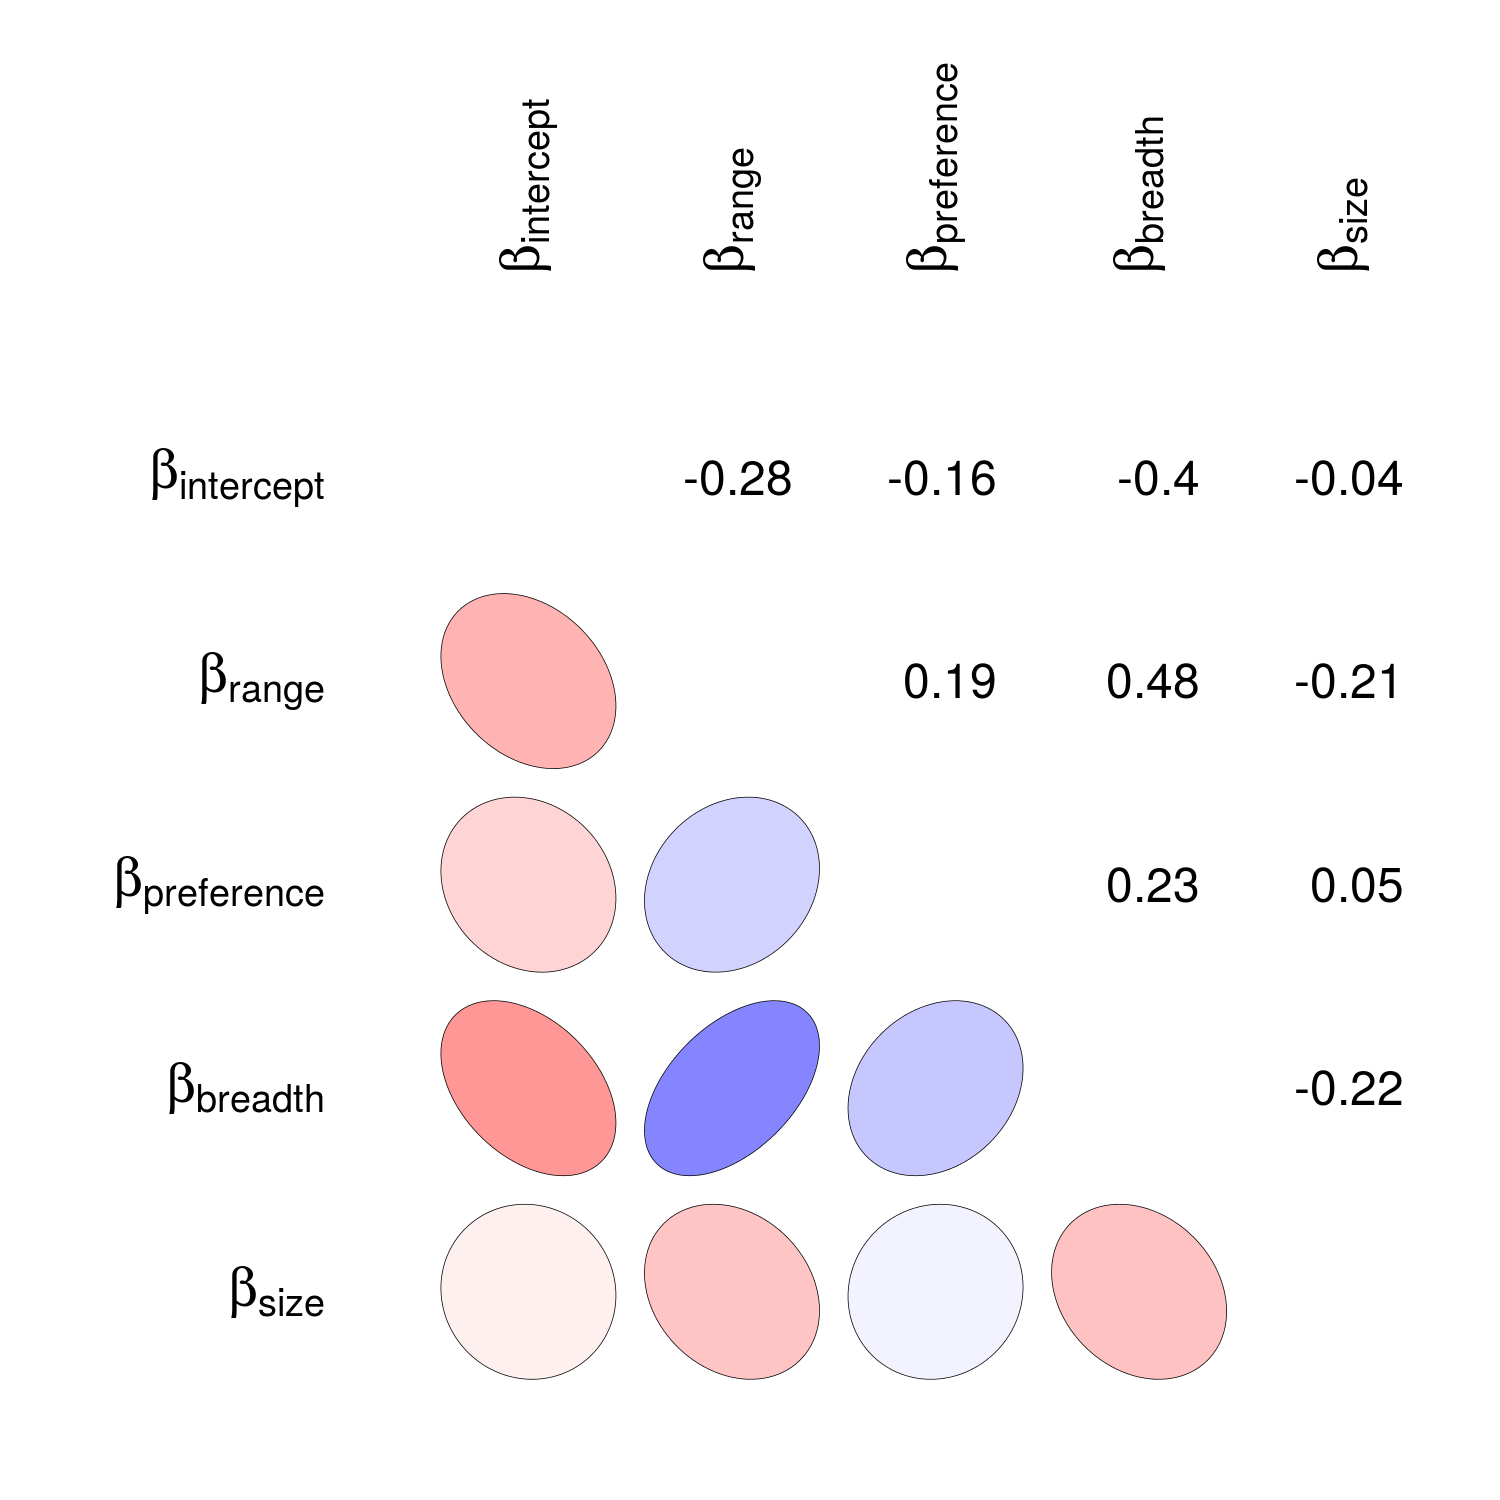
\includegraphics[height = 0.5\textheight,width=\textwidth,keepaspectratio=true]{figure/wei_cor_heatmap}
    \label{fig:omega}
  \end{subfigure}
  \begin{subfigure}[b]{0.4\textwidth}
    \caption{}
    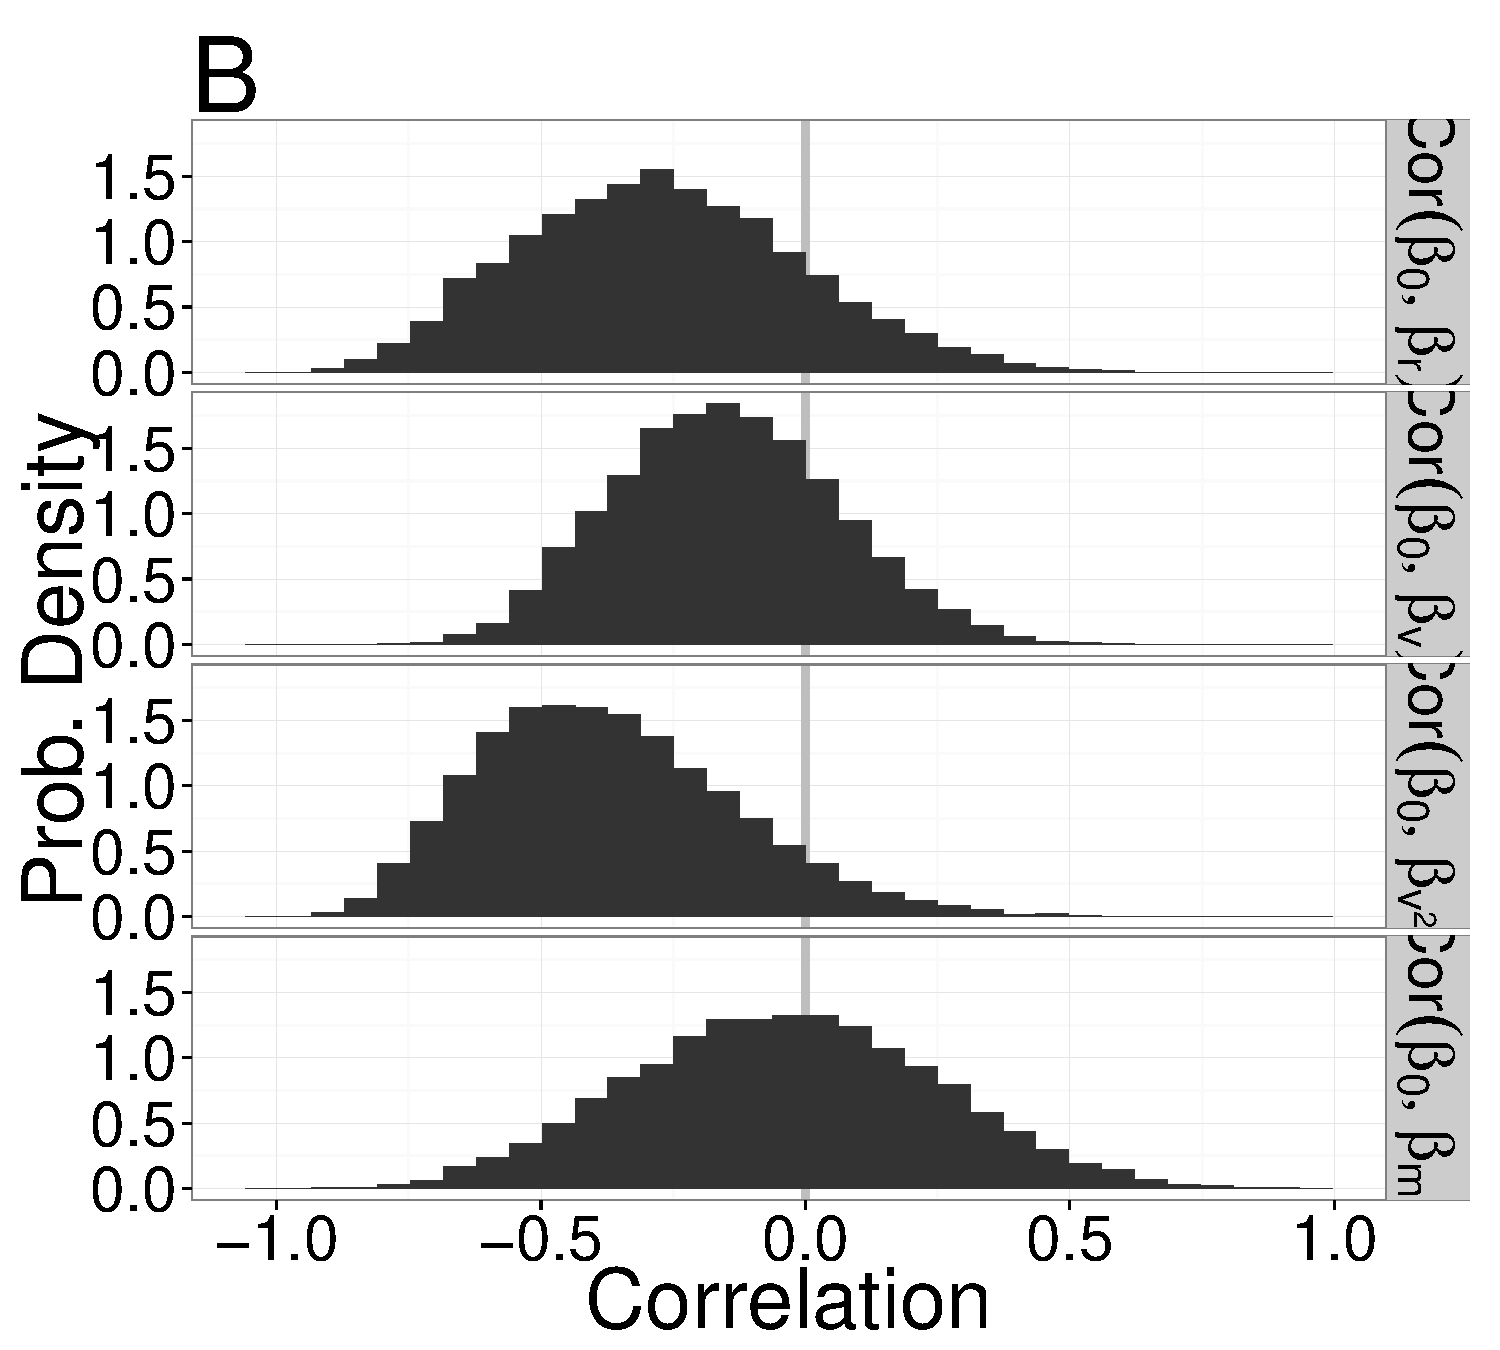
\includegraphics[height = 0.5\textheight,width=\textwidth,keepaspectratio=true]{figure/correlation_marginal}
    \label{fig:corr}
  \end{subfigure}
  \caption{\textbf{A}: Heatmap for the median estimates of the terms of the correlation matrix \(\Omega\) between cohort-level covariate effects. Both the exponential (left) and Weibull (right) models are presented. The off-diagonal terms are the correlation between the estimates of the cohort-level estimates of the effects of covariates, along with intercept/baseline extinction risk. \textbf{B}: Marginal posterior distributions of the correlations between intercept terms/baseline extinction risk and the effects of each of the covariates. These are presented for both the exponential (left) and Weibull (right) models.}
  \label{fig:cor_posterior}
\end{figure}


\begin{figure}[ht]
  \centering
  \begin{subfigure}[b]{\textwidth}
    \caption{}
    \includegraphics[width = \textwidth,keepaspectratio=true]{figure/intercept_cohort}
    \label{fig:cohort_intercept}
  \end{subfigure}

  \begin{subfigure}[b]{\textwidth}
    \caption{}
    \includegraphics[width = \textwidth,keepaspectratio=true]{figure/range_cohort}
    \label{fig:cohort_range}
  \end{subfigure}
  \caption{Comparison of cohort-specific estimates of \(\beta_{0}\) presented along with the estimate for the overall baseline extinction risk. Points correspond to the median of the cohort-specific estimate, along with 80\% credible intervals. The horizontal line is the median estimate of the overall baseline extinction risk along with 80\% credible intervals. Results are presented for the exponential (top) and Weibull (bottom) models. Comparison of cohort-specific estimates of the effect of geographic range on extinction risk \(\beta_{r}\) presented along with the estimate for the overall effect of geographic range. Points correspond to the median of the cohort-specific estimate, along with 80\% credible intervals. The horizontal line is the median estimate of the overall baseline extinction risk along with 80\% credible intervals. Results are presented for the exponential (top) and Weibull (bottom) models.}
  \label{fig:cohort_info}
\end{figure}


\begin{sidewaysfigure}[ht]
  \centering
  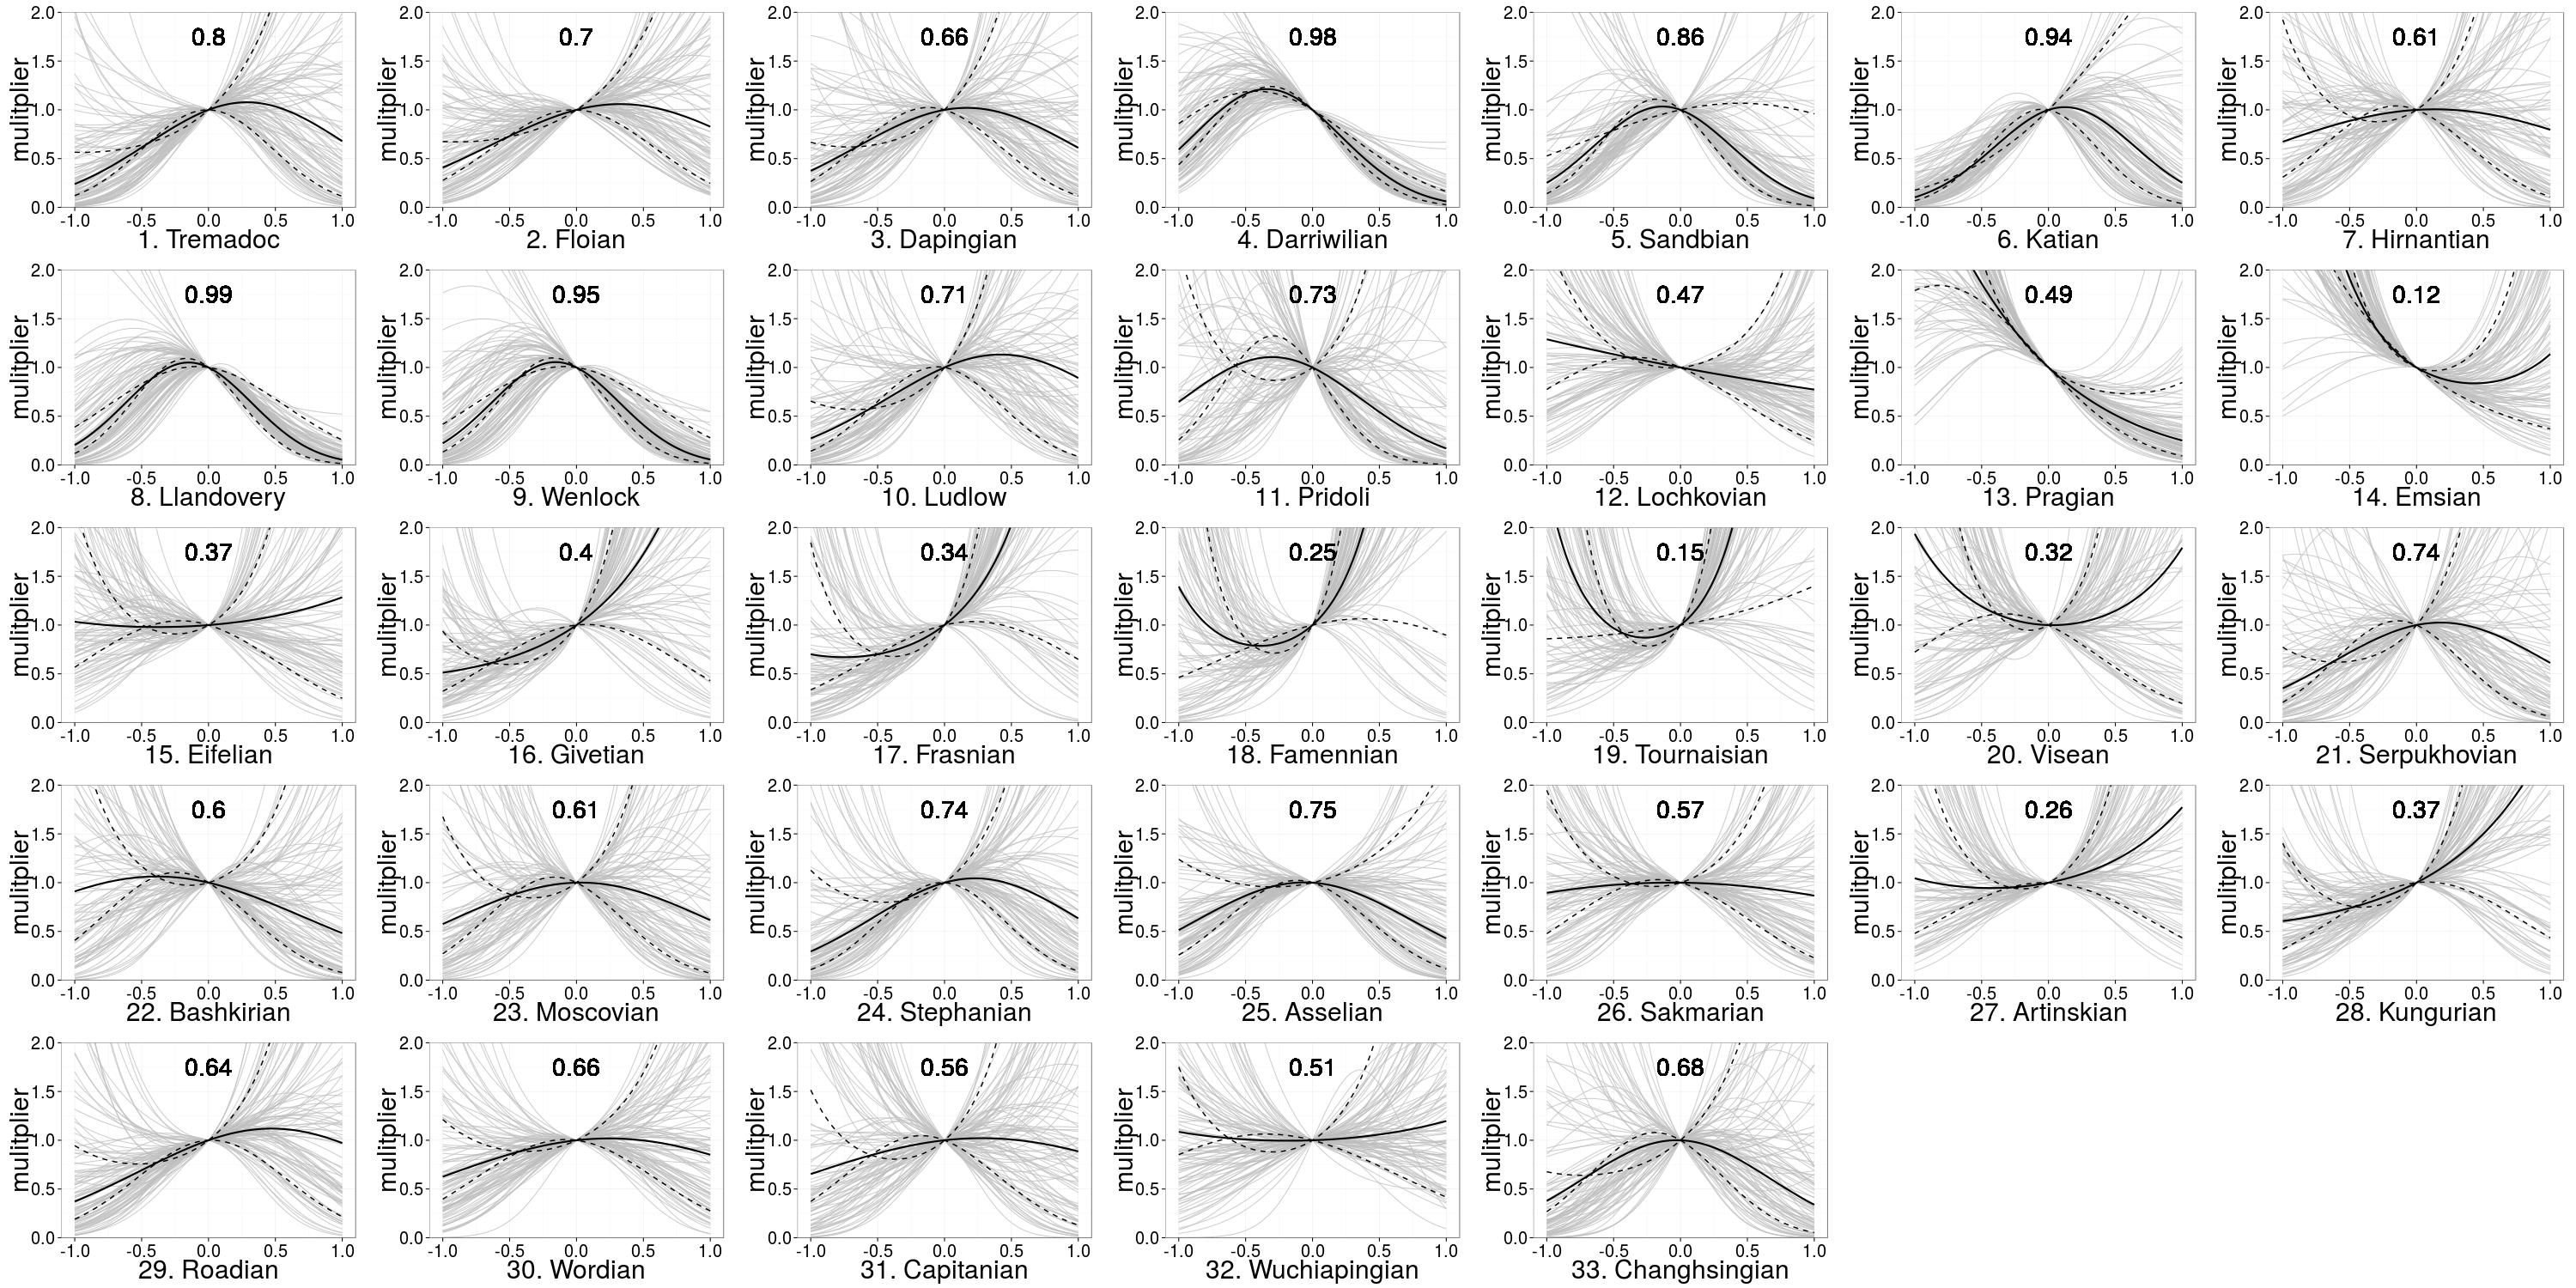
\includegraphics[height = 0.5\textheight,width=\textwidth,keepaspectratio=true]{figure/cohort_quads}
  \caption{Comparison of the cohort-specific estimates of \(f(v_{i})\) (Eq. \ref{eq:env}) for the 33 analyzed origination cohorts. The stage of origination is labeled on the x-axis of each panel. The oldest stage is in the upper left, while the youngest is in the lower left. The number in each panel corresponds to the posterior probability that \(f(v_{i})\) is concave down. Those that are highlighed in red have less than 51\% posterior predictive probability that \(f(v_{i})\) is concave down.}
  \label{fig:env_cohort}
\end{sidewaysfigure}

\begin{table}
  \centering
  \begin{tabular}{ l r r }
    \hline
    parameter & mean & standard deviation \\ 
    \hline
    \(\mu_{i}\) & -1.51 & 0.15 \\ 
    \(\mu_{r}\) & -1.38 & 0.14 \\ 
    \(\mu_{e}\) & -0.08 & 0.18 \\ 
    \(\mu_{e2}\) & 0.25 & 0.43 \\ 
    \(\mu_{m}\) & -0.09 & 0.09 \\ 
    \(\tau_{i}\) & 0.63 & 0.11 \\ 
    \(\tau_{r}\) & 0.48 & 0.12 \\ 
    \(\tau_{e}\) & 1.07 & 0.23 \\ 
    \(\tau_{e^{2}}\) & 1.88 & 0.66 \\ 
    \(\tau_{m}\) & 0.32 & 0.13 \\ 
    \hline
  \end{tabular}
  \caption{Group-level estimates of the intercept terms the effects of biological traits on brachiopod generic survival from equations \ref{eq:exp_total} and \ref{eq:wei_total}, presented as means and standard deviations. \(\mu\) values are the location parameters of the effects, while \(\tau\) values are the scale terms describing the variation between cohorts. The subscripts correspond to the following: \(i\) intercept, \(r\) geographic range, \(e\) environmental affinity, \(e^{2}\) environmental affinity squared, \(m\) body size.}
  \label{tab:param}
\end{table}

\clearpage

\appendix
\documentclass[12pt,letterpaper]{article}

\usepackage{amsmath, amsthm}
\usepackage{microtype, parskip}
\usepackage[comma,numbers,sort&compress]{natbib}
\usepackage{lineno}
\usepackage{docmute}
\usepackage{caption, subcaption, multirow, morefloats, rotating}
\usepackage{wrapfig}

\frenchspacing

\captionsetup[subfigure]{position = top, labelfont = bf, textfont = normalfont, singlelinecheck = off, justification = raggedright}

\begin{document}

\end{document}



\end{document}
